\documentclass[border=10pt]{standalone}
\usepackage{tikz}
\usetikzlibrary{arrows.meta, positioning, decorations.pathreplacing, calc}

\definecolor{convblue}{HTML}{0077B6}
\definecolor{agentamber}{HTML}{E8B517}
\definecolor{hybridgreen}{HTML}{2D6A4F}
\definecolor{txtgray}{HTML}{4A4A4A}

% 24-stop HSL-interpolated gradient (blue -> forest green -> yellow)
\definecolor{spec0}{HTML}{0077B6}
\definecolor{spec1}{HTML}{047FB0}
\definecolor{spec2}{HTML}{0886A9}
\definecolor{spec3}{HTML}{0B8CA3}
\definecolor{spec4}{HTML}{0F919C}
\definecolor{spec5}{HTML}{139496}
\definecolor{spec6}{HTML}{16908A}
\definecolor{spec7}{HTML}{1A8A7D}
\definecolor{spec8}{HTML}{1D8471}
\definecolor{spec9}{HTML}{217E67}
\definecolor{spec10}{HTML}{24785E}
\definecolor{spec11}{HTML}{277256}
\definecolor{spec12}{HTML}{2D6A4F}
\definecolor{spec13}{HTML}{2A7549}
\definecolor{spec14}{HTML}{2A7F40}
\definecolor{spec15}{HTML}{298833}
\definecolor{spec16}{HTML}{2C9228}
\definecolor{spec17}{HTML}{3D9C26}
\definecolor{spec18}{HTML}{51A625}
\definecolor{spec19}{HTML}{69B123}
\definecolor{spec20}{HTML}{84BB21}
\definecolor{spec21}{HTML}{A4C61F}
\definecolor{spec22}{HTML}{C7D11C}
\definecolor{spec23}{HTML}{DCCA1A}
\definecolor{spec24}{HTML}{E8B517}

\begin{document}
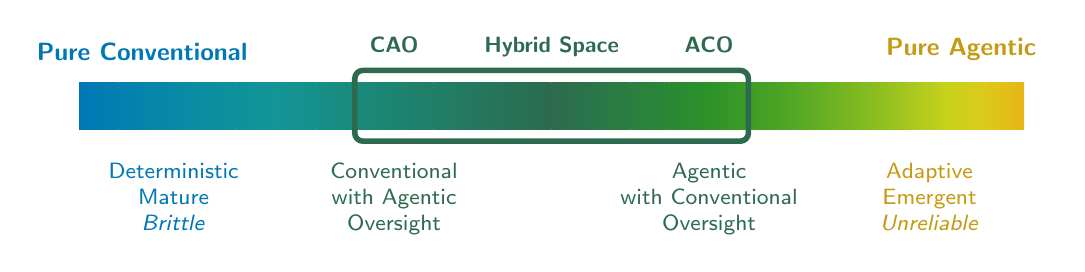
\begin{tikzpicture}[
    >=Stealth,
    font=\sffamily\small,
    text=txtgray,
]

% Spectrum bar — 24 segments for smooth pigment-mixing gradient
\shade[left color=spec0, right color=spec1] (0.0,0) rectangle (0.5,0.6);
\shade[left color=spec1, right color=spec2] (0.5,0) rectangle (1.0,0.6);
\shade[left color=spec2, right color=spec3] (1.0,0) rectangle (1.5,0.6);
\shade[left color=spec3, right color=spec4] (1.5,0) rectangle (2.0,0.6);
\shade[left color=spec4, right color=spec5] (2.0,0) rectangle (2.5,0.6);
\shade[left color=spec5, right color=spec6] (2.5,0) rectangle (3.0,0.6);
\shade[left color=spec6, right color=spec7] (3.0,0) rectangle (3.5,0.6);
\shade[left color=spec7, right color=spec8] (3.5,0) rectangle (4.0,0.6);
\shade[left color=spec8, right color=spec9] (4.0,0) rectangle (4.5,0.6);
\shade[left color=spec9, right color=spec10] (4.5,0) rectangle (5.0,0.6);
\shade[left color=spec10, right color=spec11] (5.0,0) rectangle (5.5,0.6);
\shade[left color=spec11, right color=spec12] (5.5,0) rectangle (6.0,0.6);
\shade[left color=spec12, right color=spec13] (6.0,0) rectangle (6.5,0.6);
\shade[left color=spec13, right color=spec14] (6.5,0) rectangle (7.0,0.6);
\shade[left color=spec14, right color=spec15] (7.0,0) rectangle (7.5,0.6);
\shade[left color=spec15, right color=spec16] (7.5,0) rectangle (8.0,0.6);
\shade[left color=spec16, right color=spec17] (8.0,0) rectangle (8.5,0.6);
\shade[left color=spec17, right color=spec18] (8.5,0) rectangle (9.0,0.6);
\shade[left color=spec18, right color=spec19] (9.0,0) rectangle (9.5,0.6);
\shade[left color=spec19, right color=spec20] (9.5,0) rectangle (10.0,0.6);
\shade[left color=spec20, right color=spec21] (10.0,0) rectangle (10.5,0.6);
\shade[left color=spec21, right color=spec22] (10.5,0) rectangle (11.0,0.6);
\shade[left color=spec22, right color=spec23] (11.0,0) rectangle (11.5,0.6);
\shade[left color=spec23, right color=spec24] (11.5,0) rectangle (12.0,0.6);

% Hybrid zone highlight
\draw[hybridgreen, line width=2pt, rounded corners=3pt]
    (3.5,-0.15) rectangle (8.5,0.75);
\node[hybridgreen, font=\sffamily\footnotesize\bfseries] at (6,1.05)
    {Hybrid Space};

% Left label
\node[convblue, font=\sffamily\small\bfseries, anchor=south] at (0.8,0.75)
    {Pure Conventional};
\node[text=convblue, font=\sffamily\footnotesize, text width=3cm, align=center, anchor=north]
    at (1.2,-0.3) {Deterministic\\Mature\\\textit{Brittle}};

% Right label
\node[agentamber!85!black, font=\sffamily\small\bfseries, anchor=south] at (11.2,0.75)
    {Pure Agentic};
\node[text=agentamber!85!black, font=\sffamily\footnotesize, text width=3cm, align=center, anchor=north]
    at (10.8,-0.3) {Adaptive\\Emergent\\\textit{Unreliable}};

% CAO marker — near left boundary of hybrid box
\node[hybridgreen, font=\sffamily\footnotesize\bfseries, anchor=south] at (4.0,0.85) {CAO};
\node[text=hybridgreen, font=\sffamily\footnotesize, text width=3cm, align=center, anchor=north]
    at (4.0,-0.3) {Conventional\\with Agentic\\Oversight};

% ACO marker — near right boundary of hybrid box
\node[hybridgreen, font=\sffamily\footnotesize\bfseries, anchor=south] at (8.0,0.85) {ACO};
\node[text=hybridgreen, font=\sffamily\footnotesize, text width=3cm, align=center, anchor=north]
    at (8.0,-0.3) {Agentic\\with Conventional\\Oversight};

\end{tikzpicture}
\end{document}
